% !TEX program = xelatex
\documentclass{ctexart}
\usepackage{xeCJK}
\setCJKmainfont{楷体-简 黑体}
\usepackage{geometry}
\geometry{left=2.5cm,right=2.5cm}
\usepackage[colorlinks,linkcolor=blue]{hyperref}
\CTEXsetup[format={\Large\bfseries}]{section}
\usepackage{listings}
\usepackage{xcolor}
\title{
    \LARGE
    Web信息处理与应用 Lab2-1: \\
    西班牙银行机构电话营销预测  \\[280pt]
}
\author{
    张劲暾  PB16111485 
}
\begin{document}
    \maketitle
    \newpage
    \tableofcontents
    \section{数据集描述}
    \paragraph{
        UCI数据集:\href{https://archive.ics.uci.edu/ml/datasets/Bank+Marketing}{Bank Marketing Data Set }\\
        数据集一共41188条银行向用户推荐定期存款的记录,每条记录包括如下属性,其中y属性的含义是用户最终是否订购了定期存款,是需要预测的标签:
    }
    \begin{center}
        \begin{tabular}{|c|c|c|}
            \hline
            属性名称 & 类型 & 含义 \\
            \hline
            age & int & 用户的年龄 \\
            \hline
            job & str & 用户的职业 \\
            \hline
            marital & str & 用户的婚姻状况 \\
            \hline
            education & str & 用户的受教育程度 \\
            \hline
            default & str & 用户是否默认信用 \\
            \hline
            housing & str & 用户是否有房贷 \\
            \hline
            loan & str & 用户是否有个人贷款 \\
            \hline
            contact & str & 用户的联系方式类型 \\
            \hline
            month & str & 用户本年度上一次联系的月份 \\
            \hline
            day\_of\_week & str & 用户本周上一次访问的天 \\
            \hline
            duration & int & 上次联系(订购定期存款)到目前的时间 \\
            \hline
            campaign & int & 这次商业活动中联系了多少次 \\
            \hline
            pdays & int & 上次商务活动中最后一次联系到现在的天数 \\
            \hline
            previous & int & 本次商业活动前与此用户联系的次数 \\
            \hline
            poutcome & str & 上次商业活动结果 \\
            \hline
            emp.var.rate & float & 就业率 \\
            \hline
            cons.price.idx & float & 消费者价格指数 \\
            \hline
            cons.conf.idx & float & 消费者信心指数 \\
            \hline
            euribor3m & float & 欧元区同业拆借利率 \\
            \hline
            nr.employed & float & 就业人数 \\
            \hline
            y & str & 用户是否定期存款 \\
            \hline
        \end{tabular}
    \end{center}
    
    \section{数据预处理}
        \subsection{age:用户年龄}
        \paragraph{
            用户的年龄分布如图所示:
        }
        \begin{center}
            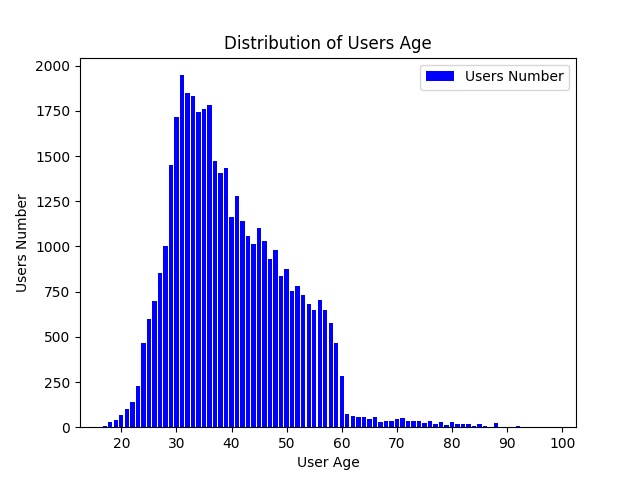
\includegraphics{age.jpg}
        \end{center}
        \paragraph{
        考虑到不同年龄段的用户需求以及人数的分布,我将年龄划分为5个区间并进行独热码编码,如表格所示:
        }
        \begin{center}
            \begin{tabular}{|c|c|}
                \hline
                年龄区间 & 独热码 \\
                \hline
                [17,25] & [0,0,0,0,1] \\
                \hline
                [25,35] & [0,0,0,1,0] \\
                \hline
                [35,45] & [0,0,1,0,0] \\
                \hline
                [45,60] & [0,1,0,0,0] \\
                \hline
                [60,98] & [1,0,0,0,0] \\
                \hline
            \end{tabular}
        \end{center}
        \subsection{job:职业}
        \paragraph{
            用户的职业分布如图所示:
        }
        \begin{center}
            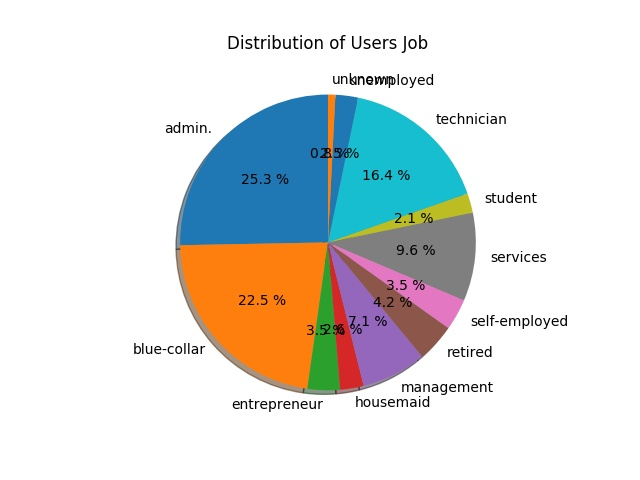
\includegraphics[height = 10.5cm]{job.jpg}
        \end{center}
        \paragraph{
            对职业进行独热码编码如表,将未知数据填充为众数:
        }
        \begin{center}
            \begin{tabular}{|c|c|}
                \hline
                职业 & 独热码 \\
                \hline
                admin.        &[0,0,0,0,0,0,0,0,0,0,1]  \\
                \hline
                blue-collar   &[0,0,0,0,0,0,0,0,0,1,0]  \\
                \hline
                entrepreneur  &[0,0,0,0,0,0,0,0,1,0,0]  \\
                \hline
                housemaid     &[0,0,0,0,0,0,0,1,0,0,0]  \\
                \hline
                management    &[0,0,0,0,0,0,1,0,0,0,0]  \\
                \hline
                retired       &[0,0,0,0,0,1,0,0,0,0,0]  \\
                \hline
                self-employed &[0,0,0,0,1,0,0,0,0,0,0]  \\
                \hline
                services      &[0,0,0,1,0,0,0,0,0,0,0]  \\
                \hline
                student       &[0,0,1,0,0,0,0,0,0,0,0]  \\
                \hline
                technician    &[0,1,0,0,0,0,0,0,0,0,0]  \\
                \hline
                unemployed    &[1,0,0,0,0,0,0,0,0,0,0]  \\
                \hline
                unknown       &[0,0,0,0,0,0,0,0,0,0,1]  \\
                \hline
            \end{tabular}
        \end{center}
        \subsection{marital:婚姻状况}
        \paragraph{
            对用户的婚姻状况进行独热码编码如表,将未知数据填充为众数:
        }
        \begin{center}
            \begin{tabular}{|c|c|}
                \hline
                婚姻状况 & 独热码 \\
                \hline
                divorced  &[0,0,1]\\
                \hline
                married   &[0,1,0]\\
                \hline
                single    &[1,0,0]\\
                \hline
                unknown   &[0,1,0]\\
                \hline
            \end{tabular}
        \end{center}
        \subsection{education:受教育程度}
        \paragraph{
            对用户的受教育程度进行独热码编码如表,将未知数据填充为众数:
        }
        \begin{center}
            \begin{tabular}{|c|c|}
                \hline
                受教育程度 & 独热码 \\
                \hline
                basic.4y              &[0,0,0,0,0,0,1]\\
                \hline
                basic.6y              &[0,0,0,0,0,1,0]\\
                \hline
                basic.9y              &[0,0,0,0,1,0,0]\\
                \hline
                high.school           &[0,0,0,1,0,0,0]\\
                \hline
                illiterate            &[0,0,1,0,0,0,0]\\
                \hline
                professional.course   &[0,1,0,0,0,0,0]\\
                \hline
                university.degree     &[1,0,0,0,0,0,0]\\
                \hline
                unknown               &[1,0,0,0,0,0,0]\\
                \hline
            \end{tabular}
        \end{center}
        \subsection{default:是否默认信用}
        \paragraph{
            这一项表示的是用户是否默认信用,绝大多数(41185条)都是没有或未知,直接放弃
        }
        \subsection{housing:是否有房贷}
        \paragraph{
            用 0 表示没有房贷, 1 表示有房贷, 缺失数据默认填充为 1。
        }
        \subsection{loan:是否有个人贷款}
        \paragraph{
            用 0 表示没有个人贷款, 1 表示有个人贷款, 缺失数据默认填充为 0。
        }
        \subsection{contact:联系方式类型}
        \paragraph{
            用 0 表示固定电话联系方式, 用 1 表示移动电话联系方式。
        }
        \subsection{month:本年度上一次联系的月份}
        \paragraph{
            这一项数据不便表示为”某种度量上的距离“,这对KNN算法和LogisticRegression算法是非常不友好的,所以我最终选择放弃这一项数据,
            试验结果表明这是有助于预测结果的准确率提高的。
        }
        \subsection{day\_of\_week:本周上一次访问的天}
        \paragraph{
            这一项数据不便表示为”某种度量上的距离“,这对KNN算法和LogisticRegression算法是非常不友好的,所以我最终选择放弃这一项数据,
            试验结果表明这是有助于预测结果的准确率提高的。
        }
        \subsection{duration:上次联系到目前的时间}
        \paragraph{
            这一项在数据集中说明有规则关系 duration = 0 ===> y = 'yes', 所以是不能使用的项。
        }
        \subsection{campaign:这次商业活动中联系了多少次}
        \paragraph{
            这一项不做离散化处理,但观察到分布为长尾趋势,所以特征值取为log2(1 + n)。
        }

        \subsection{pdays:上次商务活动中最后一次联系到现在的天数}
        \paragraph{
            这一项绝大多数是无意义的999,直接放弃。
        }
        
        \subsection{previous:本次商业活动前与此用户联系的次数}
        \paragraph{
            这一项不做离散化处理,但观察到分布为长尾趋势,所以特征值取为log2(1 + n)。
        }

        \subsection{poutcome:上次商业活动结果}
        \paragraph{
            用 -1 表示 'failure',用 0 表示 'nonexistent',用 1 表示 'success'。
        }
        \subsection{emp.var.rate:就业率}
        \paragraph{
            实值直接作为特征值。
        }
        \subsection{cons.price.idx:消费者价格指数}
        \paragraph{
            实值正则化。
        }
        \subsection{cons.conf.idx:消费者信心指数}
        \paragraph{
            实值正则化。
        }
        \subsection{euribor3m:欧元区同业拆借利率}
        \paragraph{
            实值正则化。
        }
        \subsection{nr.employed:就业人数}
        \paragraph{
            实值正则化。
        }
        \subsection{y:用户是否定期存款}
        \paragraph{
            在LogisticRegression算法中,将 ‘yes’ 转换为1,‘no’ 状换为0,方便计算。
        }
    \section{KNN算法}
    \paragraph{
        有了预处理到得到的特征向量,在本数据集上运行KNN算法的基本步骤如下:\\[20pt]  
    }
    \begin{lstlisting}[language=python, basicstyle=\small,keywordstyle=\color{blue!100},commentstyle=\color{red!100!},frame=shadowbox, rulesepcolor=\color{red!20!green!20!blue!20}]
        def KnnClassifier(TrainX,TrainY,TargetX,K):
        '''
            knn分类器:(输入输出类型均为numpy.array)
            输入:
                TrainX:训练数据集特征向量集合
                TrainY:训练数据集标签集合,与特征向量集合顺序相同
                TargetX:预测数据集特征向量集合
                K:考虑最邻近的K个点
            输出:
                TargetY:预测数据集标签集合,与特征向量集合顺序相同
        '''
        if(TrainX.shape[0] != TrainY.shape[0]):
            raise TypeError("TrainX should have same size with TrainY.")
        TargetY = []
        for i in range(TargetX.shape[0]):
            DifferentMatrix = np.tile(TargetX[i],(TrainX.shape[0],1)) - TrainX
            DiffSquarMatrix = DifferentMatrix ** 2
            Distance = DiffSquarMatrix.sum(axis = 1) ** 0.5
            DistanceSortedOrder = Distance.argsort()
            NeighLabelCount = {}
            for i in range(1,K + 1):
                NeighLabel = TrainY[DistanceSortedOrder[i]]
                NeighLabelCount[NeighLabel] = 
                NeighLabelCount.get(NeighLabel,0) + 
                ClassWeight[NeighLabel] / ( 1 + Distance[DistanceSortedOrder[i]] )
            SortedClassCount = 
            sorted(NeighLabelCount.items(),key = lambda x:x[1],reverse = True)
            TargetY.append(SortedClassCount[0][0])
        return TargetY
    \end{lstlisting}
    \section{LogisticRegression算法}
    \paragraph{
        有了预处理到得到的特征向量,在本数据集上运行LogisticRegression算法的主要学习步骤如下:
    }
    \begin{lstlisting}[language=python, basicstyle=\small, keywordstyle=\color{blue!100},commentstyle=\color{red!100!},frame=shadowbox, rulesepcolor=\color{red!20!green!20!blue!20}]
    def fit(self,X,Y):
        '''
             拟合训练数据X,Y
        '''
        if(X.shape[0] != Y.shape[0]):
            raise TypeError("X should have same size with Y.")
        self.FeatureNum = X.shape[1]
        self.InstanceNum = X.shape[0]
        self.PredictProba = np.zeros(self.InstanceNum)
        self.FeatureWeight = np.zeros(self.FeatureNum)
        for i in range(self.MaxIterTimes):
            self.PredictProba = self.get_proba(X)
            WeightAveDiff = 
            (1.0 / self.InstanceNum) * np.dot(X.T, (self.PredictProba - Y))
            WeightAveDiff += 
            ( (self.RegulizationCoef * self.FeatureWeight) / self.InstanceNum )
            self.FeatureWeight -= self.LearningtRate * WeightAveDiff
            loss = np.linalg.norm(WeightAveDiff)
            if loss < self.StopThreshold:
                break
            if i % 2500 == 0:
                print("Iteration " + str(i) + " , loss = " + str(loss))
        \end{lstlisting}
    \section{测试结果与分析}
    \subsection{KNN算法运行结果与解读}
    \paragraph{
        对于不同的K值,运行结果如下:
    }
    \begin{center}
        \begin{tabular}{|c|c|c|c|c|}
            \hline
            K & Precision & Recall & F1-score & Accuracy \\
            \hline
            1 & 0.32748538011695905 & 0.30601092896174864 & 0.3163841807909605 & 0.8483709273182958 \\
            \hline
            2 & 0.2857142857142857 & 0.45901639344262296 & 0.35220125786163525 & 0.806390977443609\\
            \hline
            3 & 0.24743589743589745 & 0.5273224043715847 & 0.33682373472949395 & 0.7619047619047619\\
            \hline
            4 & 0.2372340425531915 & 0.6092896174863388 & 0.34150076569678406 & 0.7305764411027569\\
            \hline
            5 & 0.22482893450635386 &  0.6284153005464481 & 0.3311735061195104 & 0.7089598997493735\\
            \hline
            6 & 0.25769230769230766 & 0.5491803278688525 & 0.3507853403141361 & 0.7669172932330827\\
            \hline
            7 & 0.30976430976430974 & 0.5027322404371585 & 0.3833333333333333 & 0.8145363408521303\\
            \hline
            8 & 0.31789137380191695 & 0.5437158469945356 & 0.40120967741935487 & 0.8139097744360902\\
            \hline
            9 & 0.31101190476190477 & 0.5710382513661202 & 0.4026974951830443 & 0.8057644110275689\\
            \hline
            10 & 0.30939226519337015 & 0.6120218579234973 & 0.4110091743119266 & 0.7988721804511278\\
            \hline
            11 & 0.31129476584022037 & 0.6174863387978142 & 0.41391941391941395 & 0.7994987468671679\\
            \hline
            12 & 0.32248062015503876 & 0.5683060109289617 & 0.4114737883283877 & 0.8135964912280702\\
            \hline
            13 & 0.3441780821917808 & 0.5491803278688525 & 0.4231578947368421 & 0.8283208020050126\\
            \hline
            14 & 0.34390651085141904 & 0.5628415300546448 & 0.42694300518134715 & 0.8267543859649122\\
            \hline
        \end{tabular}
    \end{center}
    \paragraph{
        可以看到在K大于10以后,基本上满足 Precision > 0.3, Recall > 0.5, F1-score值基本维持在0.4左右,Accuracy值基本维持在0.8以上,
        而y的比例大概是7:1,也就是说,KNN分类的结果大概把选择的用户订购的概率提高了三倍,涵盖了一半以上潜在的会订购定期存款的用户,还是很有意义的。
    }
    \subsection{LogisticRegression算法运行结果与解读}
    \paragraph{
        经过大量调参之后,获得的最佳结果与相应的参数如下所示:\\
        LogisticRegressionClassifier(LearningtRate=0.05,JudgeThreshold=0.25,MaxIterTimes=20000) \\
        Precision = 0.46647230320699706, Recall = 0.4371584699453552, \\
        F1-score = 0.45133991537376583, Accuracy = 0.8781328320802005\\
        可以看到对于用户订购意愿预测的准确性比KNN低,但召回率却比较低,与Random Result相比
        大概把选择的用户订购的概率提高了四倍,涵盖了百分之四十以上潜在的会订购定期存款的用户,还是很有意义的。
    }
\end{document}